\documentclass[10pt,a4paper]{article}
\usepackage[margin=1in,left=0.8in,right=0.8in]{geometry}
\usepackage{graphicx}

\title{YOLOv3 Study Notes}
\author{
Ching-Cheong Lee
}
\date{\today}
\usepackage{hyperref}
\usepackage{listings}
\usepackage{xcolor}
\usepackage{xparse}
\usepackage{amssymb,amsmath}
\usepackage{fancybox}
\usepackage{fancyvrb}


\usepackage[AutoFakeBold,AutoFakeSlant]{xeCJK}
\setCJKmainfont{Microsoft JhengHei}
\usepackage{titlesec}
\titleformat{\chapter}[display]
{\normalfont\sffamily\huge\bfseries}
{\chaptertitlename\ \thechapter}{20pt}{\Huge}
\titleformat{\section}
{\normalfont\sffamily\Large\bfseries}
{\thesection}{1em}{}


\usepackage[math-style=ISO]{unicode-math}
\xeCJKsetup{CJKmath=true}
\setmainfont{XITS}
[    Extension = .otf,
   UprightFont = *-Regular,
      BoldFont = *-Bold,
    ItalicFont = *-Italic,
BoldItalicFont = *-BoldItalic,
]
\setmathfont{XITSMath-Regular}
[    Extension = .otf,
      BoldFont = XITSMath-Bold,
]
% \setmathfont[slash-delimiter=frac]{Cambria Math}
% \setmathfont[range=up]{Cambria}
% \setmathfont[range=it]{Cambria Italic}
% \setmathfont[range=bfup]{Cambria Bold}
% \setmathfont[range=bfit]{Cambria Bold Italic}



\NewDocumentCommand{\code}{v}{%
\texttt{#1}%
}

% \newcommand{\Code}[1]{
% \VerbatimEnvironment
% \begin{BVerbatim}
% #1
% \end{BVerbatim}
% }

\newenvironment{codeblock}
{\VerbatimEnvironment
\begin{BVerbatim}}
{\end{BVerbatim}}



\definecolor{codegreen}{rgb}{0,0.6,0}
\definecolor{codegray}{rgb}{0.5,0.5,0.5}
\definecolor{codepurple}{rgb}{0.58,0,0.82}
\definecolor{backcolour}{rgb}{0.95,0.95,0.92}

\lstdefinestyle{mystyle}{
    backgroundcolor=\color{backcolour},   
    commentstyle=\color{codegreen},
    keywordstyle=\color{magenta},
    numberstyle=\tiny\color{codegray},
    stringstyle=\color{codepurple},
    basicstyle=\ttfamily\footnotesize,
    breakatwhitespace=false,         
    breaklines=true,                
    captionpos=b,                    
    keepspaces=true,                 
    numbers=none,                    
    numbersep=5pt,                  
    showspaces=false,                
    showstringspaces=false,
    showtabs=false,                  
    tabsize=2
}



\lstnewenvironment{py}{\lstset{
    language=Python,
    style=mystyle,
    breaklines=true,
    postbreak=\mbox{\textcolor{red}{$\hookrightarrow$}\space}
    }}{}

\newcommand{\END}{\text{}\hfill$\ovalbox{\small\text{\bfseries\sffamily {\itshape End} of Function}}$\bigskip}


\begin{document}
\maketitle
\section{dataset.py}

\begin{py}
def parse_annotation(self, annotation):
    line = annotation.split()
    image_path = line[0]
    if not os.path.exists(image_path):
        raise KeyError("%s does not exist ... " % imagparse_annotation
        
        e_path)
    image = cv2.imread(image_path)
    bboxes = np.array([list(map(int, box.split(','))) for box in line[1:]])

    if self.data_aug:
        image, bboxes = self.random_horizontal_flip(np.copy(image), np.copy(bboxes))
        image, bboxes = self.random_crop(np.copy(image), np.copy(bboxes))
        image, bboxes = self.random_translate(np.copy(image), np.copy(bboxes))

    image = cv2.cvtColor(image, cv2.COLOR_BGR2RGB)
    image, bboxes = utils.image_preporcess(np.copy(image), [self.train_input_size, self.train_input_size], np.copy(bboxes))
    return image, bboxes
    line = annotation.split()
    image_path = line[0]
    if not os.path.exists(image_path):
        raise KeyError("%s does not exist ... " % image_path)
    image = cv2.imread(image_path)
    bboxes = np.array([list(map(int, box.split(','))) for box in line[1:]])

    if self.data_aug:
        image, bboxes = self.random_horizontal_flip(np.copy(image), np.copy(bboxes))
        image, bboxes = self.random_crop(np.copy(image), np.copy(bboxes))
        image, bboxes = self.random_translate(np.copy(image), np.copy(bboxes))

    image = cv2.cvtColor(image, cv2.COLOR_BGR2RGB)
    image, bboxes = utils.image_preporcess(np.copy(image), [self.train_input_size, self.train_input_size], np.copy(bboxes))
    return image, bboxes
\end{py}
This part is straightfoward. \END


\begin{py}
def bbox_iou(self, boxes1, boxes2):

    boxes1 = np.array(boxes1)
    boxes2 = np.array(boxes2)

    boxes1_area = boxes1[..., 2] * boxes1[..., 3]
    boxes2_area = boxes2[..., 2] * boxes2[..., 3]

    boxes1 = np.concatenate([boxes1[..., :2] - boxes1[..., 2:] * 0.5,
                             boxes1[..., :2] + boxes1[..., 2:] * 0.5], axis=-1)
    boxes2 = np.concatenate([boxes2[..., :2] - boxes2[..., 2:] * 0.5,
                             boxes2[..., :2] + boxes2[..., 2:] * 0.5], axis=-1)
\end{py}
From the function we can deduce that $\code{box}=(c_x,c_y,\text{width},\text{height})$, therefore \[
\code{boxes[...,:2]} -  \code{boxes[...,2:]}*0.5 = \code{[all upper-left corners]}
\]
and 
\[
    \code{boxes1[..., :2]} + \code{boxes1[..., 2:]} * 0.5=\code{[all lower-right corners]},
\] while concatenating $(2,)$ \code{np}-array  along the last axis simpliy means combing them into one $(4,)$ \code{np}-array. Numerically in training \code{boxes1} and \code{boxes2} are like: \[
    \code{[[0.59375 3.78125 0.5     0.625  ]]}  
\]
and
\[
\begin{codeblock}
[[ 0.5      3.5      3.625    2.8125 ]
 [ 0.5      3.5      4.875    6.1875 ]
 [ 0.5      3.5     11.65625 10.1875 ]]
\end{codeblock}
.\] 

\begin{py}
    left_up = np.maximum(boxes1[..., :2], boxes2[..., :2])
    right_down = np.minimum(boxes1[..., 2:], boxes2[..., 2:])
\end{py}
Think of the above as entrywise comparisons that give an array of maximum, which yields the coordinates of intersection rectangle for each fixed \code{boxes1} to boxes in \code{boxes2}.
\begin{py}
    inter_section = np.maximum(right_down - left_up, 0.0)
\end{py}
The entries in \code{inter_section} are the \textit{width} and \textit{height} of the intersection, the (broadcasted) \code{np.maximum} is just a tricky way to handle empty intersection.
\begin{py}
    inter_area = inter_section[..., 0] * inter_section[..., 1]
    union_area = boxes1_area + boxes2_area - inter_area

    return inter_area / union_area
\end{py}


\END


\begin{py}
def preprocess_true_boxes(self, bboxes):
\end{py}

Here \code{bboxes} are the boxes from annotation file in which each line takes the form:
\[
\code{some/directory/hash.jpg 79,537,107,574,0 297,547,318,575,0}
\]

\begin{py}
    label = [np.zeros((self.train_output_sizes[i],
                       self.train_output_sizes[i],
                       self.anchor_per_scale,
                       5 + self.num_classes)) for i in range(3)]
    bboxes_xywh = [np.zeros((self.max_bbox_per_scale, 4)) for _ in range(3)]
    bbox_count = np.zeros((3,))

    for bbox in bboxes:
        bbox_coor = bbox[:4]
        bbox_class_ind = bbox[4]

        onehot = np.zeros(self.num_classes, dtype=np.float)
        onehot[bbox_class_ind] = 1.0
        uniform_distribution = np.full(self.num_classes, 1.0 / self.num_classes)
        deta = 0.01
        smooth_onehot = onehot * (1 - deta) + deta * uniform_distribution
        # bbox_xywh is ground truth
        bbox_xywh = np.concatenate([(bbox_coor[2:] + bbox_coor[:2]) * 0.5, bbox_coor[2:] - bbox_coor[:2]], axis=-1)
        # bbox_xywh_scaled is scaled ground truth relative to stride (13, 26, 52, as a unit)
        bbox_xywh_scaled = 1.0 * bbox_xywh[np.newaxis, :] / self.strides[:, np.newaxis]
\end{py}
Note that \code{bbox_xywh[np.newaxis, :]} is of shape \code{(1, 4)} and \code{1/self.strides[:, np.newaxis]} is of shape \code{(3, 1)}, their multiplication will be conducted by ``broadcasting'' in \code{numpy}, which yields a $(3, 4)$  dimensional \code{numpy} array. The product \code{bbox_xywh_scaled} consists of $(c_x,c_y,w,h)$ which use ``stride'' as a unit, so 1 means ``1 grid'' (recall there are $13\times 13$, $26\times 26$, $52\times 52$ grids predictions from Darknet backbone).
\begin{py}
        iou = []
        exist_positive = False
        for i in range(3):
            anchors_xywh = np.zeros((self.anchor_per_scale, 4))
            anchors_xywh[:, 0:2] = np.floor(bbox_xywh_scaled[i, 0:2]).astype(np.int32) + 0.5
            anchors_xywh[:, 2:4] = self.anchors[i]
\end{py}
\code{anchors_xywh} essing boxes with objectiveneentially move centers of \code{bbox_xywh_scaled} to the middle of the grid that center lies in, then the anchor boxes' width and height are assigned, replacing the original width, height of \code{bbox_xywh_scaled}.
\begin{py}
            iou_scale = self.bbox_iou(bbox_xywh_scaled[i][np.newaxis, :], anchors_xywh)
\end{py}
The presence of \code{np.newaxis} is simply because multiplication between $(4,)$  and $(3,4)$ array does not make sense. The additional dimension expand $(4,)$ array into $(1,4)$ array, which is broadcasted and multiplied to $(3,4)$ array to give anothoer $(3,4)$ array, and theirfore, $\code{iou_scale.shape} = (3, )$.
\begin{py}
            iou.append(iou_scale)
            iou_mask = iou_scale > 0.3 # a boolean list of length 3

            if np.any(iou_mask): # if one of them is True
                xind, yind = np.floor(bbox_xywh_scaled[i, 0:2]).astype(np.int32)
                label[i][yind, xind, iou_mask, :] = 0
                label[i][yind, xind, iou_mask, 0:4] = bbox_xywh
                label[i][yind, xind, iou_mask, 4:5] = 1.0
                label[i][yind, xind, iou_mask, 5:] = smooth_onehot
\end{py}
% self.train_output_sizes = self.train_input_size // self.strides
\code{label[i]} is initialized at the beginning which is of size 
\[\code{train_output_sizes}\times \code{train_output_sizes}\times 3\times 85\]
for each \code{i}, where $\code{train_output_sizes} = 13,26$ or $52$. 
\begin{py}
                bbox_ind = int(bbox_count[i] % self.max_bbox_per_scale)
                bboxes_xywh[i][bbox_ind, :4] = bbox_xywh
\end{py}
\code{bboxes_xywh} is initialized (with zeros) at the beginning, $\code{bboxes_xywh.shape} = (3,150,4)$.
\begin{py}
                bbox_count[i] += 1

                exist_positive = True

        if not exist_positive:
            best_anchor_ind = np.argmax(np.array(iou).reshape(-1), axis=-1) # flatten and take max
            # best_detect belongs to which "i", namely, best "i"
            best_detect = int(best_anchor_ind / self.anchor_per_scale)
            # for this i, which index it is:
            best_anchor = int(best_anchor_ind % self.anchor_per_scale)
            # get the grid point in our 13x13, 26x26, 52x52 grid:
            xind, yind = np.floor(bbox_xywh_scaled[best_detect, 0:2]).astype(np.int32)

            label[best_detect][yind, xind, best_anchor, :] = 0
            label[best_detect][yind, xind, best_anchor, 0:4] = bbox_xywh
            label[best_detect][yind, xind, best_anchor, 4:5] = 1.0
            label[best_detect][yind, xind, best_anchor, 5:] = smooth_onehot

            bbox_ind = int(bbox_count[best_detect] % self.max_bbox_per_scale)
            bboxes_xywh[best_detect][bbox_ind, :4] = bbox_xywh 
            # assign bbox_xywh into the list instead of append, 
            # this is to make sure there are at most 150 boxes within all 3 scales.   

            bbox_count[best_detect] += 1
    label_sbbox, label_mbbox, label_lbbox = label
    sbboxes, mbboxes, lbboxes = bboxes_xywh
    return label_sbbox, label_mbbox, label_lbbox, sbboxes, mbboxes, lbboxes
\end{py}
In short, \[\code{sbboxes, mbboxes, lbboxe}\] 
are just ground truth bounding boxes (center, width and height), while \[\code{label_sbbox, label_mbbox, label_lbbox}\] are ground truth bounding boxes with objectiveness and probabilities of \textbf{\textit{each grid}}.
\END

\section{yolov3.py}

In \code{darknet53} after a bunch of residue modules we get 3 branches \code{route_1}, \code{route_2} and \code{cov}, where
\begin{center}
\begin{minipage}{\textwidth}
\[\code{route_1.shape}= (-1,52,52,256)\]
\[\code{route_2.shape} = (-1,26,26, 512) \]
\[\code{conv.shape} =(-1,13,13,1024) \]
\end{minipage}
\end{center}
\begin{figure}
\centering
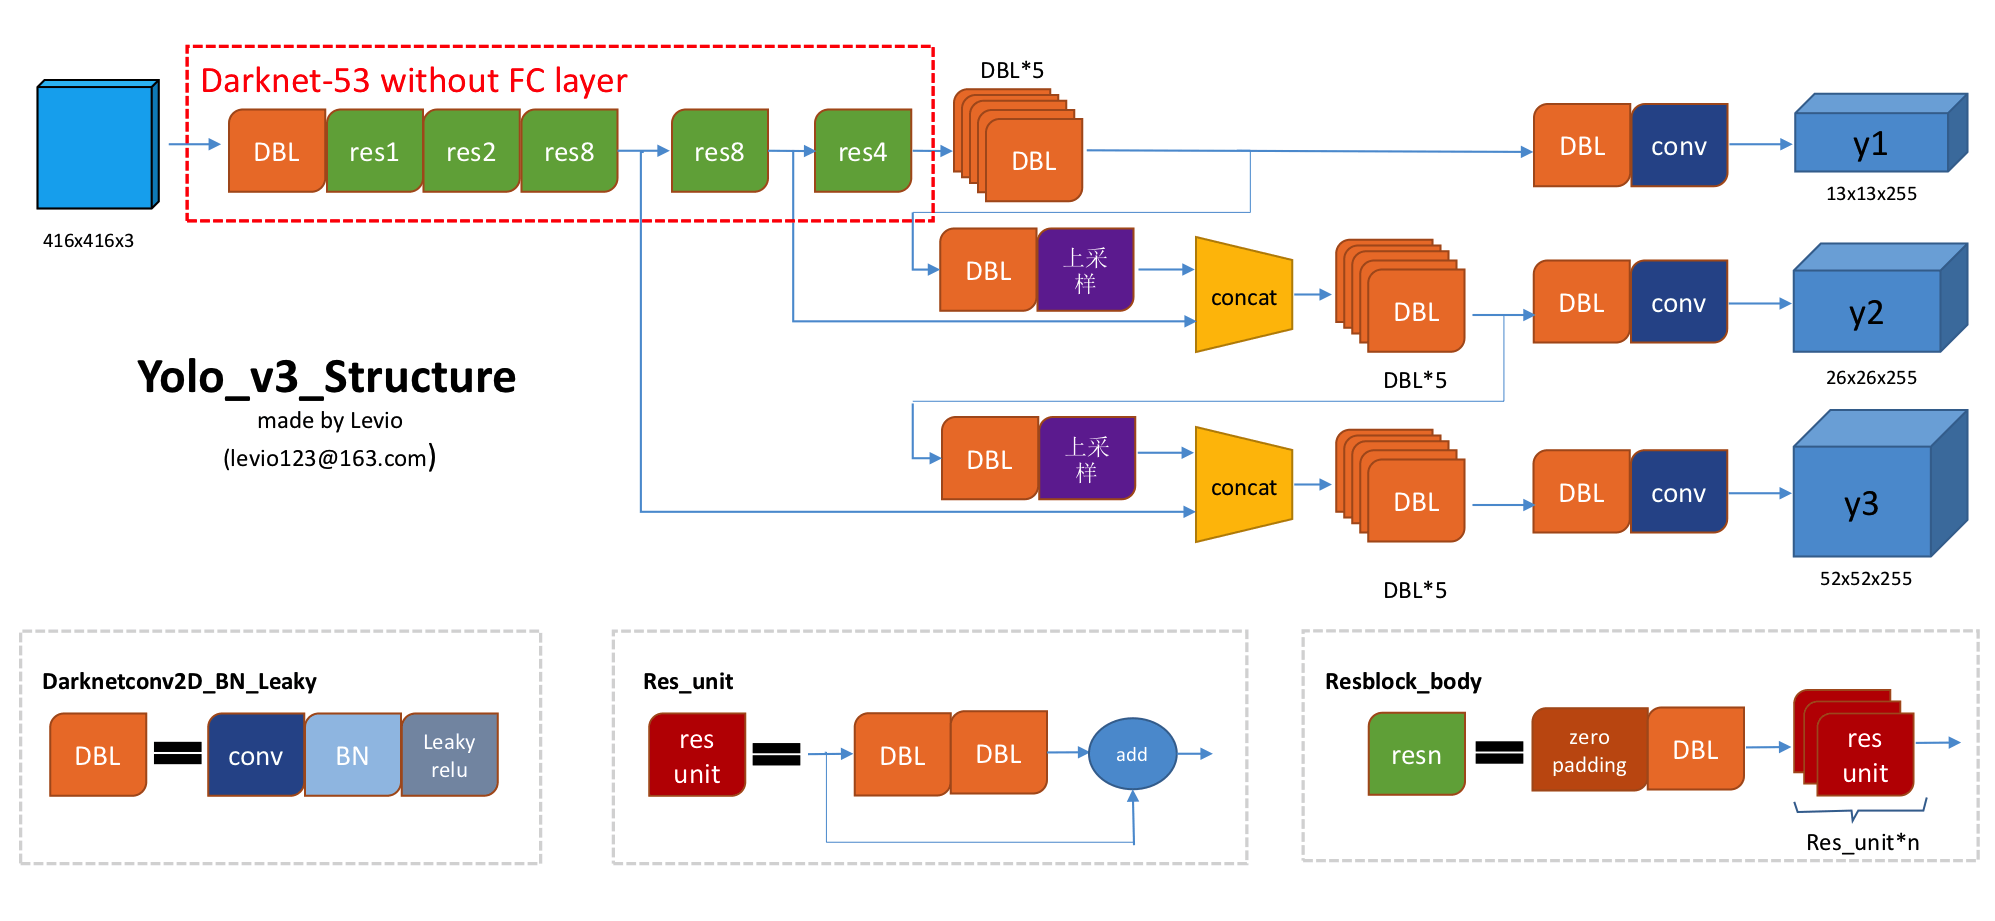
\includegraphics[width=\textwidth]{./yolo_structure.png}
\caption{Structure of YOLOv3}
\end{figure} 

Each branch then jumps into several stages of feature extractions, the whole process finally gives another 3 branches of undecoded/raw data of features, and they are endowed with the meaning of ``grid-based detection'' after reshaping into $(-1,\code{output_size},\code{output_size}, 3, 85 )$ dimensional array.

\begin{py}
def YOLOv3(input_layer):
    route_1, route_2, conv = backbone.darknet53(input_layer)

    conv = common.convolutional(conv, (1, 1, 1024,  512))
    conv = common.convolutional(conv, (3, 3,  512, 1024))
    conv = common.convolutional(conv, (1, 1, 1024,  512))
    conv = common.convolutional(conv, (3, 3,  512, 1024))
    conv = common.convolutional(conv, (1, 1, 1024,  512))
\end{py}
As \code{padding="same"} is being used along the chain of conv nets, there is no spatial dimension change.
\begin{py}
    conv_lobj_branch = common.convolutional(conv, (3, 3, 512, 1024))
    conv_lbbox = common.convolutional(conv_lobj_branch, (1, 1, 1024, 3*(NUM_CLASS + 5)), activate=False, bn=False)

    conv = common.convolutional(conv, (1, 1,  512,  256))
    conv = common.upsample(conv)

    conv = tf.concat([conv, route_2], axis=-1)

    conv = common.convolutional(conv, (1, 1, 768, 256))
    conv = common.convolutional(conv, (3, 3, 256, 512))
    conv = common.convolutional(conv, (1, 1, 512, 256))
    conv = common.convolutional(conv, (3, 3, 256, 512))
    conv = common.convolutional(conv, (1, 1, 512, 256))

    conv_mobj_branch = common.convolutional(conv, (3, 3, 256, 512))
    conv_mbbox = common.convolutional(conv_mobj_branch, (1, 1, 512, 3*(NUM_CLASS + 5)), activate=False, bn=False)

    conv = common.convolutional(conv, (1, 1, 256, 128))
    conv = common.upsample(conv)

    conv = tf.concat([conv, route_1], axis=-1)

    conv = common.convolutional(conv, (1, 1, 384, 128))
    conv = common.convolutional(conv, (3, 3, 128, 256))
    conv = common.convolutional(conv, (1, 1, 256, 128))
    conv = common.convolutional(conv, (3, 3, 128, 256))
    conv = common.convolutional(conv, (1, 1, 256, 128))

    conv_sobj_branch = common.convolutional(conv, (3, 3, 128, 256))
    conv_sbbox = common.convolutional(conv_sobj_branch, (1, 1, 256, 3*(NUM_CLASS +5)), activate=False, bn=False)

    return [conv_sbbox, conv_mbbox, conv_lbbox]
\end{py}
\END


\begin{py}
def decode(conv_output, i=0):
    """
    return tensor of shape [batch_size, output_size, output_size, anchor_per_scale, 5 + num_classes]
            contains (x, y, w, h, score, probability)
    """
\end{py}
\code{conv_output} is the output of \code{YOLOv3} (\code{conv_sbbox}, \code{conv_mbbox} or \code{conv_lbbox}).
\begin{py}
    conv_shape       = tf.shape(conv_output)
    batch_size       = conv_shape[0]
    output_size      = conv_shape[1]

    conv_output = tf.reshape(conv_output, (batch_size, output_size, output_size, 3, 5 + NUM_CLASS))

    conv_raw_dxdy = conv_output[:, :, :, :, 0:2]
    conv_raw_dwdh = conv_output[:, :, :, :, 2:4]
    conv_raw_conf = conv_output[:, :, :, :, 4:5]
    conv_raw_prob = conv_output[:, :, :, :, 5: ]

    y = tf.tile(tf.range(output_size, dtype=tf.int32)[:, tf.newaxis], [1, output_size])
    x = tf.tile(tf.range(output_size, dtype=tf.int32)[tf.newaxis, :], [output_size, 1])
\end{py}
For example, let's take $\code{output_size}=13$, then \[\code{y = np.tile(np.arange(13)[:, np.newaxis], [1, 13])}\] and \[\code{x = np.tile(np.arange(13)[np.newaxis, :], [13, 1])}\]
are respectively:
\[
\begin{codeblock}
[[ 0  0  0  0  0  0  0  0  0  0  0  0  0]   [[ 0  1  2  3  4  5  6  7  8  9 10 11 12]
 [ 1  1  1  1  1  1  1  1  1  1  1  1  1]    [ 0  1  2  3  4  5  6  7  8  9 10 11 12]
 [ 2  2  2  2  2  2  2  2  2  2  2  2  2]    [ 0  1  2  3  4  5  6  7  8  9 10 11 12]
 [ 3  3  3  3  3  3  3  3  3  3  3  3  3]    [ 0  1  2  3  4  5  6  7  8  9 10 11 12]
 [ 4  4  4  4  4  4  4  4  4  4  4  4  4]    [ 0  1  2  3  4  5  6  7  8  9 10 11 12]
 [ 5  5  5  5  5  5  5  5  5  5  5  5  5]    [ 0  1  2  3  4  5  6  7  8  9 10 11 12]
 [ 6  6  6  6  6  6  6  6  6  6  6  6  6]    [ 0  1  2  3  4  5  6  7  8  9 10 11 12]
 [ 7  7  7  7  7  7  7  7  7  7  7  7  7]    [ 0  1  2  3  4  5  6  7  8  9 10 11 12]
 [ 8  8  8  8  8  8  8  8  8  8  8  8  8]    [ 0  1  2  3  4  5  6  7  8  9 10 11 12]
 [ 9  9  9  9  9  9  9  9  9  9  9  9  9]    [ 0  1  2  3  4  5  6  7  8  9 10 11 12]
 [10 10 10 10 10 10 10 10 10 10 10 10 10]    [ 0  1  2  3  4  5  6  7  8  9 10 11 12]
 [11 11 11 11 11 11 11 11 11 11 11 11 11]    [ 0  1  2  3  4  5  6  7  8  9 10 11 12]
 [12 12 12 12 12 12 12 12 12 12 12 12 12]]   [ 0  1  2  3  4  5  6  7  8  9 10 11 12]]
\end{codeblock}
\]
For \code{x} and \code{y} we expand dimension again along the last axis (break every single element into a bracketed element) before concatenation:
\begin{py}
    xy_grid = tf.concat([x[:, :, tf.newaxis], y[:, :, tf.newaxis]], axis=-1)
\end{py}
At this point, \code{xy_grid} is $(13,13,2)$ dimensional.
\begin{py}
    xy_grid = tf.tile(xy_grid[tf.newaxis, :, :, tf.newaxis, :], [batch_size, 1, 1, 3, 1])
    xy_grid = tf.cast(xy_grid, tf.float32)
\end{py}
Now \code{xy_grid} is $(\code{batch_size}, 13, 13, 3, 2)$ dimensional. Recall that 
\begin{center}
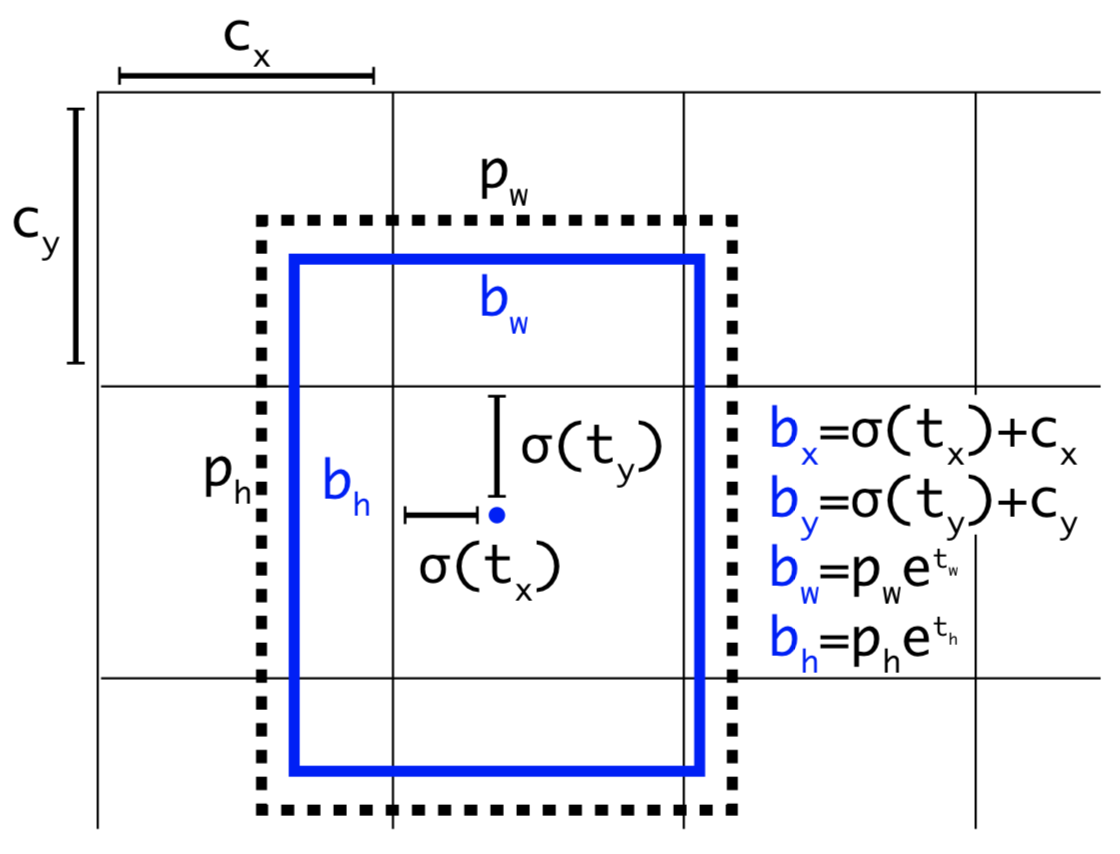
\includegraphics[width=0.3\textwidth]{./decode_anchor.png}
\end{center}
\begin{py}
    pred_xy = (tf.sigmoid(conv_raw_dxdy) + xy_grid) * STRIDES[i]
    pred_wh = (tf.exp(conv_raw_dwdh) * ANCHORS[i]) * STRIDES[i]
    pred_xywh = tf.concat([pred_xy, pred_wh], axis=-1)

    pred_conf = tf.sigmoid(conv_raw_conf)
    pred_prob = tf.sigmoid(conv_raw_prob)

    return tf.concat([pred_xywh, pred_conf, pred_prob], axis=-1)
\end{py}
Bear in mind that decoded \code{x}, \code{y} in \code{pred_xywh} denote the center of prediction rectangle, as is the output of the function \code{preprocess_true_boxes}. \END



\section{yolov3.compute\_loss}

\begin{py}
def bbox_giou(boxes1, boxes2):

    boxes1 = tf.concat([boxes1[..., :2] - boxes1[..., 2:] * 0.5,
                        boxes1[..., :2] + boxes1[..., 2:] * 0.5], axis=-1)
    boxes2 = tf.concat([boxes2[..., :2] - boxes2[..., 2:] * 0.5,
                        boxes2[..., :2] + boxes2[..., 2:] * 0.5], axis=-1)

    boxes1 = tf.concat([tf.minimum(boxes1[..., :2], boxes1[..., 2:]),
                        tf.maximum(boxes1[..., :2], boxes1[..., 2:])], axis=-1)
    boxes2 = tf.concat([tf.minimum(boxes2[..., :2], boxes2[..., 2:]),
                        tf.maximum(boxes2[..., :2], boxes2[..., 2:])], axis=-1)

    boxes1_area = (boxes1[..., 2] - boxes1[..., 0]) * (boxes1[..., 3] - boxes1[..., 1])
    boxes2_area = (boxes2[..., 2] - boxes2[..., 0]) * (boxes2[..., 3] - boxes2[..., 1])

    left_up = tf.maximum(boxes1[..., :2], boxes2[..., :2])
    right_down = tf.minimum(boxes1[..., 2:], boxes2[..., 2:])

    inter_section = tf.maximum(right_down - left_up, 0.0)
    inter_area = inter_section[..., 0] * inter_section[..., 1]
    union_area = boxes1_area + boxes2_area - inter_area
    iou = inter_area / union_area

    enclose_left_up = tf.minimum(boxes1[..., :2], boxes2[..., :2])
    enclose_right_down = tf.maximum(boxes1[..., 2:], boxes2[..., 2:])
    enclose = tf.maximum(enclose_right_down - enclose_left_up, 0.0)
    enclose_area = enclose[..., 0] * enclose[..., 1]
    giou = iou - 1.0 * (enclose_area - union_area) / enclose_area

    return giou
\end{py}




\begin{py}
def compute_loss(pred, conv, label, bboxes, i=0):

    conv_shape  = tf.shape(conv)
    batch_size  = conv_shape[0]
    output_size = conv_shape[1]
    input_size  = STRIDES[i] * output_size
    conv = tf.reshape(conv, (batch_size, output_size, output_size, 3, 5 + NUM_CLASS))

    conv_raw_conf = conv[:, :, :, :, 4:5]
    conv_raw_prob = conv[:, :, :, :, 5:]

    pred_xywh     = pred[:, :, :, :, 0:4]
    pred_conf     = pred[:, :, :, :, 4:5]

    label_xywh    = label[:, :, :, :, 0:4]
    respond_bbox  = label[:, :, :, :, 4:5] # objectiveness
    label_prob    = label[:, :, :, :, 5:]

    giou = tf.expand_dims(bbox_giou(pred_xywh, label_xywh), axis=-1)
    input_size = tf.cast(input_size, tf.float32)

    bbox_loss_scale = 2.0 - 1.0 * label_xywh[:, :, :, :, 2:3] * label_xywh[:, :, :, :, 3:4] / (input_size ** 2)
    giou_loss = respond_bbox * bbox_loss_scale * (1- giou)
\end{py}
Note that for two sets $U,V\in \mathcal C$, where $\mathcal C\in 2^{\mathbb R^2}$, the function $d(U,V) := 1-\text{giou}(U,V)$ defines a metric, so \code{giou_loss} makes sense.
\begin{py}
    iou = bbox_iou(pred_xywh[:, :, :, :, np.newaxis, :], bboxes[:, np.newaxis, np.newaxis, np.newaxis, :, :])
\end{py}
\code{bboxes} are batched inside \code{Dataset("train").__next__} before passing into \code{compute_loss} (in a while loop until image count reaches batch size). Therefore $\code{bboxes.shape} = (16, 150, 4)$, where $150$ is the maximal number of anchors (most of them are zeros due to initialization), so we see 3 \code{:}'s in \code{bboxes}. 

Finally 
\[\code{pred_xywh.shape}=(16, 13,13,3,150,4)=\code{bboxes.shape}\]
and \[\code{iou.shape} = (16,13,13,3,150)\]
where computation gets rid of the last dimension. \code{bboxes} is copied to every grid for computation because from original paper:
\bigskip
\begin{center}\itshape
   ``the confidence prediction represents the IOU between the predicted box and any ground truth box"
\end{center}
\begin{py}
    max_iou = tf.expand_dims(tf.reduce_max(iou, axis=-1), axis=-1)
    respond_bgd = (1.0 - respond_bbox) * tf.cast( max_iou < IOU_LOSS_THRESH, tf.float32 )
\end{py}
In the internet some people call \code{IOU_LOSS_THRESH} as \code{ignore_thresh}. \code{respond_bgd} determines whether to penalize a prediction  
\begin{itemize}
\item that overlaps too few with ground truth anchors (i.e., detected wrong location) \textit{\bfseries and} 
\item that makes false positive error.
\end{itemize}
\begin{py}
    conf_focal = tf.pow(respond_bbox - pred_conf, 2)
\end{py}
The concept of focal loss with $\gamma = 2$ was introduced in \cite{focalLoss}, which down-weights the loss contributed by well-classificed (high confidence) examples.
\begin{py}
    conf_loss = conf_focal *
    (
        respond_bbox * tf.nn.sigmoid_cross_entropy_with_logits(labels=respond_bbox, logits=conv_raw_conf)
        +
        respond_bgd * tf.nn.sigmoid_cross_entropy_with_logits(labels=respond_bbox, logits=conv_raw_conf)
    )
\end{py}
Where \code{tf.nn.sigmoid_cross_entropy_with_logits(labels=z, logits=x)} is 
\[\code{z * -log(sigmoid(x)) + (1 - z) * -log(1 - sigmoid(x))},\]
therefore \code{x} has to be a raw prediction data.
\begin{py}
    prob_loss = respond_bbox * tf.nn.sigmoid_cross_entropy_with_logits(labels=label_prob, logits=conv_raw_prob)

    giou_loss = tf.reduce_mean(tf.reduce_sum(giou_loss, axis=[1,2,3,4]))
    conf_loss = tf.reduce_mean(tf.reduce_sum(conf_loss, axis=[1,2,3,4]))
    prob_loss = tf.reduce_mean(tf.reduce_sum(prob_loss, axis=[1,2,3,4]))

    return giou_loss, conf_loss, prob_loss
\end{py}
\END

\section{train.py}
\textbf{Recap of Customized Training Loop with GradientTape.} Apart from predefined loss functions (such as \code{categorical_crossentropy} for classfication, \code{mse} for regression, etc), it is ocassional to come across non-standard loss functions from other repository with the use of \code{tf.GradientTape}. 

Such implementation usually create 4 components:

\begin{description}
    \item[Component 1.] The model \textbf{architecture}
    \item[Component 2.] The \textbf{loss function} used when computing the model loss
    \item[Component 3.]  The \textbf{optimizer} used to update the model weights
    \item[Component 4.] The \textbf{step function} that encapsulates the forward and backward pass of the network
\end{description}

Now the code below is self-explanatory:

\begin{py}
def train_step(image_data, target, epoch):

    # image_data = batch of images

    with tf.GradientTape() as tape:
        pred_result = model(image_data, training=True)
        giou_loss = conf_loss = prob_loss = 0

        # optimizing process
        for i in range(3):
            conv, pred = pred_result[i*2], pred_result[i*2+1]
            batch_label, batch_bboxes = target[i]
            loss_items = compute_loss(pred, conv, batch_label, batch_bboxes, i)
            giou_loss += loss_items[0]
            conf_loss += loss_items[1]
            prob_loss += loss_items[2]

        total_loss = giou_loss + conf_loss + prob_loss

        gradients = tape.gradient(total_loss, model.trainable_variables)
        optimizer.apply_gradients(zip(gradients, model.trainable_variables))

        # update learning rate
        global_steps.assign_add(1)
        if global_steps < warmup_steps:
            lr = global_steps / warmup_steps * cfg.TRAIN.LR_INIT
        else:
            lr = cfg.TRAIN.LR_END + 0.5 * (cfg.TRAIN.LR_INIT - cfg.TRAIN.LR_END) * (
                (1 + tf.cos((global_steps - warmup_steps) / (total_steps - warmup_steps) * np.pi))
            )
        optimizer.lr.assign(lr.numpy())

        # writing summary data
        with writer.as_default():
            tf.summary.scalar("lr", optimizer.lr, step=global_steps)
            tf.summary.scalar("loss/total_loss", total_loss, step=global_steps)
            tf.summary.scalar("loss/giou_loss", giou_loss, step=global_steps)
            tf.summary.scalar("loss/conf_loss", conf_loss, step=global_steps)
            tf.summary.scalar("loss/prob_loss", prob_loss, step=global_steps)
        writer.flush()

for epoch in range(cfg.TRAIN.EPOCHS):
    for index, (image_data, target) in enumerate(trainset):
        train_step(image_data, target, epoch)

    model.save_weights("./checkpoints/yolov3-{}-{}.h5".format(cfg.WEIGHT_NAME_TO_SAVE, epoch))
\end{py}









\begin{thebibliography}{9}
    \bibitem{yoloanalysis1to5} 
    \textit{YOLOv3源码解析 1-5}, \url{https://blog.csdn.net/sxlsxl119/article/details/103028021}.

    \bibitem{yunyang}
    \textit{YOLOv3 算法的一点理解}, \url{https://yunyang1994.gitee.io/2018/12/28/YOLOv3/}.

    \bibitem{focalLoss} Tsung-Yi Lin, Priya Goyal, Ross Girshick, Kaiming He and  Piotr Dollar, \textit{Focal Loss for Dense Object Detection}, \url{https://arxiv.org/pdf/1708.02002.pdf?fbclid=IwAR38T65chV0UNPhBDbAExH021_afC0L6o9PEztpBPBAzqY3dBR8vOGy2qwg}. 

    \bibitem{yolov3} Joseph Redmon, Ali Farhadi, YOLOv3: \textit{An Incremental Improvement}, \url{https://arxiv.org/abs/1804.02767}.
    
    \bibitem{pyimgsearch} Adrian Rosebrock, \textit{Using TensorFlow and GradientTape to train a Keras model}, \url{https://www.pyimagesearch.com/2020/03/23/using-tensorflow-and-gradienttape-to-train-a-keras-model/}
\end{thebibliography}



\end{document}


